\documentclass{beamer}
\usepackage{listings}
\usepackage{hyperref}
\usepackage{tikz}
\usetikzlibrary{positioning,shadows,arrows,shapes,calc}
\usepackage{tipa}
\newcommand{\ipa}[1]{\fontfamily{cmr}\selectfont\textipa{#1}}
\def\labelenumi\theenumi
\usepackage{graphicx}
\usepackage{amsmath}
\mode<presentation>{\usetheme{Frankfurt}}
\AtBeginSection
{
  \begin{frame}<beamer>
    \frametitle{Outline}
    \tableofcontents[currentsection,currentsubsection]
  \end{frame}
}
\title{Long/Short-Term Memory}
\author{Mark Hasegawa-Johnson\\All content~\href{https://creativecommons.org/licenses/by-sa/4.0/}{CC-SA 4.0} unless otherwise specified.}
\date{ECE 417: Multimedia Signal Processing, Fall 2020}  
\institute{University of Illinois}
\titlegraphic{\includegraphics{../../../17fall/lectures/imark_1867_bold.png}}
\begin{document}

% Title
\begin{frame}
  \maketitle
\end{frame}

% Title
\begin{frame}
  \tableofcontents
\end{frame}


%%%%%%%%%%%%%%%%%%%%%%%%%%%%%%%%%%%%%%%%%%%%%%%%%%%%%%%%%
\section[Review]{Review: Recurrent Neural Networks}
\setcounter{subsection}{1}

\begin{frame}
  \frametitle{Recurrent Neural Net (RNN) = Nonlinear(IIR)}
  \centerline{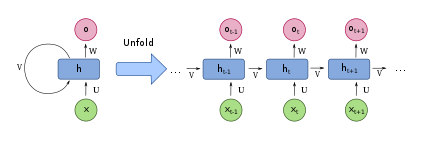
\includegraphics[width=4.5in]{../lec18/Recurrent.png}}
  \begin{tiny}Image CC-SA-4.0  by Ixnay, \url{https://commons.wikimedia.org/wiki/File:Recurrent_neural_network_unfold.svg}\end{tiny}
\end{frame}

\begin{frame}
  \frametitle{Back-Propagation and Causal Graphs}

  \centerline{
    \tikzstyle{pre}=[<-,shorten <=1pt,>=stealth',semithick,draw=blue]
    \begin{tikzpicture}[hoop/.style={circle,thick,draw=blue,text=black,
          fill=orange!35!white,text centered,text width=0.25cm}]
      \node[hoop] (x) at (0,0) {$x$};
      \node[hoop] (h0) at (-2,1) {$h_0$} edge[pre] (x);
      \node[hoop] (h1) at (2,2) {$h_1$} edge[pre] (x) edge[pre](h0);
      \draw[dashed] (-2.5,0.5) -- (2.5,0.5);
      \node[hoop] (yhat) at (0,3) {$\hat{y}$} edge[pre](h0) edge[pre](h1);
  \end{tikzpicture}}
  \begin{displaymath}
    \frac{d\hat{y}}{dx} = \sum_{i=0}^{N-1}\frac{d\hat{y}}{dh_i}\frac{\partial h_i}{\partial x}
  \end{displaymath}
  For each $h_i$, we find the {\bf total derivative} of $\hat{y}$
  w.r.t. $h_i$, multiplied by the {\bf partial derivative} of $h_i$ w.r.t. $x$.
\end{frame}

\begin{frame}
  \frametitle{Back-Propagation Through Time}
  Back-propagation through time computes the error gradient at
  each time step based on the error gradients at future time steps.
  If the forward-prop equation is
  \begin{displaymath}
    \hat{y}[n]=g(e[n]),~~~e[n]=x[n]+\sum_{m=1}^{M-1} w[m]\hat{y}[n-m],
  \end{displaymath}
  then the BPTT equation is
  \begin{displaymath}
    \delta[n]=\frac{dE}{de[n]}=\frac{\partial E}{\partial e[n]}+
    \sum_{m=1}^{M-1}\delta[n+m]w[m]\dot{g}(e[n])
  \end{displaymath}
  Weight update, for an RNN, multiplies the back-prop times the
  forward-prop.
  \[
  \frac{dE}{dw[m]} = \sum_n \delta[n] \hat{y}[n-m]
  \]
\end{frame}


%%%%%%%%%%%%%%%%%%%%%%%%%%%%%%%%%%%%%%%%%%%%%%%%%%%%%%%%%
\section[Vanishing Gradient]{Vanishing/Exploding Gradient}
\setcounter{subsection}{1}

\begin{frame}
  \frametitle{Vanishing/Exploding Gradient}
  \begin{itemize}
    \item The ``vanishing gradient'' problem refers to the tendency of
      $\frac{d\hat{y}[n+m]}{de[n]}$ to disappear,
      exponentially, when $m$ is large.
  \item
    The ``exploding gradient'' problem refers to the tendency of
    $\frac{d\hat{y}[n+m]}{de[n]}$ to explode toward infinity,
    exponentially, when $m$ is large.
  \item
    If the largest feedback coefficient is $|w[m]|>1$, then you get
    exploding gradient.  If $|w[m]|<1$, you get vanishing gradient.
    \end{itemize}
\end{frame}

\begin{frame}
  \frametitle{Example: A Memorizer Network}
  Suppose that we have a very simple RNN:
  \[
  \hat{y}[n] = w x[n]+u\hat{y}[n-1]
  \]
  Suppose that $x[n]$ is only nonzero at time $0$:
  \begin{align*}
    x[n]=\begin{cases}x_0&n=0\\0& n\ne 0\end{cases}
  \end{align*}
  Suppose that, instead of measuring $x[0]$ directly, we are only
  allowed to measure the output of the RNN $m$ time-steps later.  Our goal is
  to learn $w$ and $u$ so that $\hat{y}[m]$ remembers $x_0$, thus:
  \[
  E=\frac{1}{2}\left(\hat{y}[m]-x_0\right)^2
  \]
\end{frame}

\begin{frame}
  \frametitle{Example: A Memorizer Network}

  Now, how do we perform gradient update of the weights?  If
  \[
  \hat{y}[n] = w x[n]+u\hat{y}[n-1]
  \]
  then
  \begin{align*}
    \frac{dE}{dw} &= \sum_n \left(\frac{dE}{d\hat{y}[n]}\right)\frac{\partial \hat{y}[n]}{\partial w} \\
   &= \sum_n \left(\frac{dE}{d\hat{y}[n]}\right)x[n]
    = \left(\frac{dE}{d\hat{y}[0]}\right)x_0
  \end{align*}
  But the error is defined as
  \[
  E=\frac{1}{2}\left(\hat{y}[m]-x_0\right)^2
  \]
  so
  \begin{align*}
    \frac{dE}{d\hat{y}[0]} &= u\frac{dE}{d\hat{y}[1]} = u^2\frac{dE}{d\hat{y}[2]} = \ldots
    = u^m \left(\hat{y}[m]-x_0\right)
  \end{align*}
\end{frame}
  
\begin{frame}
  \begin{columns}
    \column{2.75in}
    \begin{block}{Example: Vanishing Gradient}
      So we find out that the gradient, w.r.t. the coefficient $w$, is
      either exponentially small, or exponentially large, depending on
      whether $|u|<1$ or $|u|>1$:
      \[
      \frac{dE}{dw} = x_0\left(\hat{y}[m]-x_0\right) u^m
      \]
      In other words, if our application requires the neural net to
      wait $m$ time steps before generating its output, then the
      gradient is exponentially smaller, and therefore training the
      neural net is exponentially harder.
    \end{block}
    \column{1.75in}
    \begin{block}{Exponential Decay}
      \centerline{\includegraphics[width=1.75in]{../../../18fall/lectures/l27/1920px-Plot-exponential-decay.png}}
      \begin{tiny}Image CC-SA-4.0, PeterQ, Wikipedia\end{tiny}
    \end{block}
    \end{columns}
\end{frame}

%%%%%%%%%%%%%%%%%%%%%%%%%%%%%%%%%%%%%%%%%%%%%%%%%%%%%%%%%
\section[Example]{Running Example: a Pocket Calculator}
\setcounter{subsection}{1}

\begin{frame}
  \frametitle{Notation}

  Today's lecture will try to use notation similar to the Wikipedia
  page for LSTM.
  \begin{itemize}
  \item $x[t]=$ input at time $t$
  \item $y[t]=$ target/desired output
  \item $c[t]=$ excitation at time $t$~{\bf\em OR}~LSTM cell
  \item $h[t]=$ activation at time $t$~{\bf\em OR}~LSTM output
  \item $u=$ feedback coefficient
  \item $w=$ feedforward coefficient
  \item $b=$ bias
  \end{itemize}
\end{frame}

\begin{frame}
  \frametitle{Running Example: a Pocket Calculator} The rest of this
  lecture will refer to a toy application called ``pocket calculator.''
  \begin{block}{Pocket Calculator}
    \begin{itemize}
    \item When $x[t]>0$, add it to the current tally: $c[t]=c[t-1]+x[t]$.
    \item When $x[t]=0$,
      \begin{enumerate}
      \item Print out the current tally, $h[t]=c[t-1]$, and then
      \item Reset the tally to zero, $c[t]=0$.
      \end{enumerate}
    \end{itemize}
  \end{block}
  \begin{block}{Example Signals}
    \begin{align*}
      \mbox{\bf Input:}~x[t] &= 1,2,1,0,1,1,1,0\\
      \mbox{\bf Target Output:}~y[t] &= 0,0,0,4,0,0,0,3
    \end{align*}
  \end{block}
\end{frame}

\begin{frame}  
  \begin{columns}
    \column{2in}
    \begin{block}{Pocket Calculator}
      \begin{itemize}
      \item When $x[t]>0$, add it to the current tally: $c[t]=c[t-1]+x[t]$.
      \item When $x[t]=0$,
        \begin{enumerate}
        \item Print out the current tally, $h[t]=c[t-1]$, and then
        \item Reset the tally to zero, $c[t]=0$.
        \end{enumerate}
      \end{itemize}
    \end{block}
    \column{2.25in}
    \begin{block}{Pocket Calculator}
      \centerline{\includegraphics[width=2.25in]{exp/fig0.png}}
    \end{block}
    \end{columns}
\end{frame}
  
%%%%%%%%%%%%%%%%%%%%%%%%%%%%%%%%%%%%%%%%%%%%%%%%%%%%%%%%%
\section[RNN]{Regular RNN}
\setcounter{subsection}{1}

\begin{frame}
  \frametitle{One-Node One-Tap Linear RNN}
  Suppose that we have a very simple RNN:
  \begin{align*}
    \mbox{Excitation:}~c[t] &= x[t]+uh[t-1]\\
    \mbox{Activation:}~h[t] &= \sigma_h\left(c[t]\right)
  \end{align*}
  where $\sigma_h()$ is some feedback nonlinearity.  In this simple
  example, let's just use $\sigma_h(c[t])=c[t]$, i.e., no
  nonlinearity. 

  {\bf GOAL:} Find $u$ so that $h[t]\approx
  y[t]$.  In order to make the problem easier, we will only score an
  ``error'' when $y[t]\ne 0$:
  \[
  E = \frac{1}{2}\sum_{t:y[t]>0} \left(h[t]-y[t]\right)^2
  \]
\end{frame}

\begin{frame}
  \begin{columns}
    \column{2.25in}
    \begin{block}{RNN: $u=1$?}
      Obviously, if we want to just add numbers, we should just set
      $u=1$.  Then the RNN is computing
      \begin{align*}
        \mbox{Excitation:}~c[t] &= x[t]+h[t-1]\\
        \mbox{Activation:}~h[t] &= \sigma_h\left(c[t]\right)
      \end{align*}
      That works until the first zero-valued input.  But then it just
      keeps on adding.
    \end{block}
    \column{2.25in}
    \begin{block}{RNN with $u=1$}
      \centerline{\includegraphics[width=2.25in]{exp/fig1.png}}
    \end{block}
    \end{columns}
\end{frame}

\begin{frame}
  \begin{columns}
    \column{2.25in}
    \begin{block}{RNN: $u=0.5$?}
      Can we get decent results using $u=0.5$? 
      \begin{itemize}
        \item Advantage: by the time we reach $x[t]=0$, the sum has
          kind of leaked away from us ($c[t]\approx 0$), so a
          hard-reset is not necessary.
        \item Disadvantage: by the time we reach $x[t]=0$, the sum has
          kind of leaked away from us ($h[t]\approx 0$).
      \end{itemize}
    \end{block}
    \column{2.25in}
    \begin{block}{RNN with $u=0.5$}
      \centerline{\includegraphics[width=2.25in]{exp/fig2.png}}
    \end{block}
    \end{columns}
\end{frame}

\begin{frame}
  \frametitle{Gradient Descent}

  \begin{align*}
    c[t] &= x[t]+uh[t-1]\\
    h[t] &= \sigma_h\left(c[t]\right)
  \end{align*}
  Let's try initializing $u=0.5$, and then performing gradient descent
  to improve it.  Gradient descent has five steps:
  \begin{enumerate}
  \item {\bf Forward Propagation:} $c[t]=x[t]+uh[t-1]$, $h[t]=c[t]$.
  \item {\bf Synchronous Backprop:} $\epsilon[t]=\partial E/\partial c[t]$.
  \item {\bf Back-Prop Through Time:} $\delta[t]=dE/dc[t]$.
  \item {\bf Weight Gradient:} $dE/du=\sum_t \delta[t]h[t-1]$
  \item {\bf Gradient Descent:} $u\leftarrow u-\eta dE/du$
  \end{enumerate}
\end{frame}

\begin{frame}
  \frametitle{Gradient Descent}
  \begin{align*}
    \mbox{Excitation:}~c[t] &= x[t]+uh[t-1]\\
    \mbox{Activation:}~h[t] &= \sigma_h\left(c[t]\right)\\
    \mbox{Error:}~E &= \frac{1}{2}\sum_{t:y[t]>0} \left(h[t]-y[t]\right)^2
  \end{align*}
  So the back-prop stages are:
  \begin{align*}
    \mbox{\bf Synchronous Backprop:}~\epsilon[t] &=\frac{\partial E}{\partial c[t]}=
    \left\{\begin{array}{ll} (h[t]-y[t]) & y[t]>0\\0&\mbox{otherwise}\end{array}\right.\\
    \mbox{\bf BPTT:}~\delta[t] &=\frac{dE}{dc[t]}= \epsilon[t]+u\delta[t+1]\\
    \mbox{\bf Weight Gradient:}~\frac{dE}{du}&=\sum_t \delta[t]h[t-1]
  \end{align*}
\end{frame}

\begin{frame}
  \begin{columns}
    \column{2.2in}
    \begin{block}{Backprop Stages}
      \begin{align*}
        \epsilon[t] &=
        \left\{\begin{array}{ll} (h[t]-y[t]) & y[t]>0\\0&\mbox{otherwise}\end{array}\right.\\
        \delta[t] &= \epsilon[t]+u\delta[t+1]\\
        \frac{dE}{du}&=\sum_t \delta[t]h[t-1]
      \end{align*}
    \end{block}
    \column{2.5in}
    \begin{block}{Backprop Stages, $u=0.5$}
      \centerline{\includegraphics[width=2.5in]{exp/fig3.png}}
    \end{block}
    \end{columns}
\end{frame}

\begin{frame}
  \frametitle{Vanishing Gradient and Exploding Gradient}
  \begin{itemize}
    \item Notice that, with $|u|<1$, $\delta[t]$ tends to vanish
      exponentially fast as we go backward in time.  This is called
      the {\bf vanishing gradient} problem.  It is a big problem for
      RNNs with long time-dependency, and for deep neural nets with
      many layers.
    \item If we set $|u|>1$, we get an even worse problem, sometimes
      called the {\bf exploding gradient} problem.
  \end{itemize}
\end{frame}
        
\begin{frame}
  \begin{columns}
    \column{2.25in}
    \begin{block}{RNN, $u=1.7$}
      \[
      c[t] = x[t]+uh[t-1]
      \]
      \centerline{\includegraphics[width=2.25in]{exp/fig4.png}}
    \end{block}
    \column{2.25in}
    \begin{block}{RNN, $u=1.7$}
      \[
      \delta[t]=\epsilon[t]+u\delta[t+1]
      \]
      \centerline{\includegraphics[width=2.25in]{exp/fig5.png}}
    \end{block}
    \end{columns}
\end{frame}

%%%%%%%%%%%%%%%%%%%%%%%%%%%%%%%%%%%%%%%%%%%%%%%%%%%%%%%%%%%%%%%%%%%%%%%%%%%%%%%%%
\section[Forget Gate]{Forget Gate}
\setcounter{subsection}{1}

\begin{frame}
  \frametitle{Hochreiter and Schmidhuber's Solution: The Forget Gate}

  Instead of multiplying by the same weight, $u$, at each time step,
  Hochreiter and Schmidhuber proposed: let's make the feedback
  coefficient a function of the input!
  \begin{align*}
    \mbox{Excitation:}~c[t] &= x[t]+f[t]h[t-1]\\
    \mbox{Activation:}~h[t] &= \sigma_h\left(c[t]\right)\\
    \mbox{Forget Gate:}~f[t] &= \sigma_g\left(w_fx[t]+u_fh[t-1]+b_f\right)\\
  \end{align*}
  Where $\sigma_h()$ and $\sigma_g()$ might be different
  nonlinearities.  In particular, it's OK for $\sigma_h()$ to be
  linear ($\sigma_h(c)=c$), but $\sigma_g()$ should be clipped so that
  $0\le f[t]\le 1$, in order to avoid gradient explosion.
\end{frame}

\begin{frame}
  \frametitle{The Forget-Gate Nonlinearity}
  The forget gate is
  \[
  f[t] = \sigma_g\left(w_fx[t]+u_fh[t-1]+b_f\right)
  \]
  where $\sigma_g()$ is some nonlinearity such that $0\le \sigma_g() \le
  1$.  Two such nonlinearities are worth knowing about.
\end{frame}
\begin{frame}
  \frametitle{Forget-Gate Nonlinearity \#1: CReLU}

  The first useful nonlinearity is the CReLU (clipped rectified linear
  unit), defined as
  \[
  \sigma_g(w_fx+u_fh+b_f) = \min\left(1,\max\left(0,w_fx+u_fh+b_f\right)\right)
  \]
  \begin{itemize}
    \item The CReLU is particularly useful for {\bf knowledge-based
      design}.  That's because $\sigma(1)=1$ and $\sigma(0)=0$, so it
      is relatively easy to design the weights $w_f$, $u_f$, and $b_f$
      to get the results you want.
    \item The CReLU is not very useful, though, if you want to choose
      your weights using {\bf gradient descent}.  What usually happens
      is that $w_f$ grows larger and larger for the first 2-3 epochs
      of training, and then suddenly $w_f$ is so large that
      $\dot\sigma(w_fx+u_fh+b_f)=0$ for all training tokens.  At that
      point, the gradient is $dE/dw=0$, so further gradient-descent
      training is useless.
  \end{itemize}
\end{frame}

\begin{frame}
  \frametitle{Forget-Gate Nonlinearity \#1: Logistic Sigmoid}

  The second useful nonlinearity is the logistic sigmoid, defined as:
  \[
  \sigma_g(w_fx+u_fh+b_f) = \frac{1}{1+e^{-(w_fx+u_fh+b_f)}}
  \]
  \begin{itemize}
  \item The logistic sigmoid is particularly useful for {\bf gradient
    descent}.  That's because its gradient is defined for all values
    of $w_f$.  In fact, it has a really simple form, that can be
    written in terms of the output: $\dot\sigma=\sigma(1-\sigma)$.
  \item The logistic sigmoid is not as useful for {\bf knowledge-based
    design}.  That's because $0<\sigma<1$: as $x\rightarrow -\infty$,
    $\sigma(x)\rightarrow 0$, but it never quite reaches it.  Likewise
    as $x\rightarrow\infty$, $\sigma(x)\rightarrow 1$, but it never
    quite reaches it.
  \end{itemize}
\end{frame}
\begin{frame}
  \begin{columns}
    \column{2in}
    \begin{block}{Pocket Calculator}
      \begin{itemize}
        \item When $x[t]>0$, accumulate the input, and print out
          nothing.
        \item When $x[t]=0$, print out the accumulator, then reset.
      \end{itemize}
      \ldots but the ``print out nothing'' part is not scored, only
      the accumulation.  Furthermore, nonzero input is always $x[t]\ge
      1$.
    \end{block}
    \column{2.5in}
    \begin{block}{}
      \centerline{\includegraphics[width=2.5in]{exp/fig0.png}}
    \end{block}
    \end{columns}
\end{frame}
\begin{frame}
  \begin{columns}
    \column{2in}
    \begin{block}{Pocket Calculator}
      With zero error, we can approximate the pocket calculator as
      \begin{itemize}
        \item When $x[t]\ge 1$, accumulate the input.
        \item When $x[t]=0$, print out the accumulator, then reset.
      \end{itemize}
    \end{block}
    \column{2.5in}
    \begin{block}{$E=\frac{1}{2}\sum_{t:y[t]>0} \left(h[t]-y[t]\right)^2=0$}
      \centerline{\includegraphics[width=2.5in]{exp/fig6.png}}
    \end{block}
    \end{columns}
\end{frame}
\begin{frame}
  \frametitle{Forget-Gate Implementation of the Pocket Calculator}

  It seems like we can approximate the pocket calculator as:
  \begin{itemize}
  \item When $x[t]\ge 1$, accumulate the input: $c[t]=x[t]+h[t-1]$.
  \item When $x[t]=0$, print out the accumulator, then reset: $c[t]=x[t]$.
  \end{itemize}
  So it seems that we just want the forget gate set to
  \[
  f[t]=\left\{\begin{array}{ll}
  1 & x[t]\ge 1\\
  0 & x[t]=0
  \end{array}\right.
  \]
  This can be accomplished as
  \[
  f[t]=\mbox{CReLU}\left(x[t]\right)=\max\left(0,\min\left(1,x[t]\right)\right)
  \]
\end{frame}

\begin{frame}
  \begin{columns}
    \column{2in}
    \begin{block}{Forget Gate Implementation of the Pocket Calculator}
      \begin{align*}
        c[t] &= x[t]+f[t]h[t-1]\\
        h[t] &= c[t]\\
        f[t] &= \mbox{CReLU}\left(x[t]\right)
      \end{align*}
    \end{block}
    \column{2.25in}
    \begin{block}{Forward Prop}
      \centerline{\includegraphics[width=2.25in]{exp/fig7.png}}
    \end{block}
    \end{columns}
\end{frame}

\begin{frame}
  \begin{columns}
    \column{2in}
    \begin{block}{Forget Gate Implementation of the Pocket Calculator}
      \begin{align*}
        c[t] &= x[t]+f[t]h[t-1]\\
        h[t] &= c[t]\\
        f[t] &= \mbox{CReLU}\left(x[t]\right)
      \end{align*}
    \end{block}
    \column{2.5in}
    \begin{block}{Back Prop}
      \centerline{\includegraphics[width=2.5in]{exp/fig8.png}}
    \end{block}
    \end{columns}
\end{frame}

\begin{frame}
  \frametitle{What Went Wrong?}
  \begin{itemize}
    \item The forget gate correctly turned itself on (remember the
      past) when $x[t]>0$, and turned itself off (forget the past)
      when $x[t]=0$.
    \item Unfortunately, we don't want to forget the past when
      $x[t]=0$.  We want to forget the past on the {\bf next time step
      after} $x[t]=0$.
    \item Coincidentally, we also don't want any output when $x[t]>0$.
      The error criterion doesn't score those samples, but maybe it
      should.
  \end{itemize}
\end{frame}

%%%%%%%%%%%%%%%%%%%%%%%%%%%%%%%%%%%%%%%%%%%%%%%%%%%%%%%%%%%%%%%%%%%%%%%%%%%%%%%%%
\section[LSTM]{Long Short-Term Memory (LSTM)}
\setcounter{subsection}{1}

\begin{frame}
  \frametitle{Long Short-Term Memory (LSTM)}

  The LSTM solves those problems by defining two types of memory, and
  three types of gates.  The two types of memory are
  \begin{enumerate}
  \item The ``cell,'' $c[t]$, corresponds to the excitation in an RNN.
  \item The ``output'' or ``prediction,'' $h[t]$, corresponds to the activation in an RNN.
  \end{enumerate}
  The three gates are:
  \begin{enumerate}
  \item The cell remembers the past only when the forget gate is on, $f[t]=1$.
  \item The cell accepts input only when the input gate is on, $i[t]=1$.
  \item The cell is output only when the output gate is on, $o[t]=1$.
  \end{enumerate}
\end{frame}
  
\begin{frame}
  \frametitle{Long Short-Term Memory (LSTM)}
  The three gates are:
  \begin{enumerate}
  \item The cell remembers the past only when the forget gate is on, $f[t]=1$.
  \item The cell accepts input only when the input gate is on, $i[t]=1$.
    \[
    c[t] = f[t]c[t-1] + i[t]\sigma_h\left(w_cx[t]+u_ch[t-1]+b_c\right)
    \]
  \item The cell is output only when the output gate is on, $o[t]=1$.
    \[
    h[t] = o[t]c[t]
    \]
  \end{enumerate}
\end{frame}
  
\begin{frame}
  \frametitle{Characterizing Human Memory}
  \begin{center}
    \tikzstyle{pre}=[<-,shorten <=1pt,>=stealth',semithick,draw=blue]
    \tikzstyle{post}=[->,shorten >=1pt,>=stealth',semithick,draw=blue]
    \begin{tikzpicture}[
        hoop/.style={circle,thick, draw=blue, text=black, fill=orange!35!white, text centered, text width=1.25cm},
        open/.style={circle,thick, draw=blue, text=black, text centered, text width=1cm},
        bend angle=60
      ]
      \node[hoop] (ltm) at (0,0) {LONG\\TERM};
      \node[hoop] (stm) at (4,0) {SHORT\\TERM}
      edge[pre,bend left] node[above=3.2cm,name=e1] {INPUT GATE} (ltm)
      edge[post,bend right] node[below=3.2cm,name=e2] {OUTPUT GATE} (ltm);
      \node (perception) at (8,2) {PERCEPTION} edge[post] (stm);
      \node (action) at (8,-2) {ACTION} edge[pre] (stm);
    \end{tikzpicture}
  \end{center}
  \[
  \Pr\left\{\mbox{remember}\right\}=p_{LTM} e^{-t/T_{LTM}}+ (1-p_{LTM})e^{-t/T_{STM}}
  \]
\end{frame}

\begin{frame}
  \frametitle{When Should You Remember?}
  \begin{align*}
    c[t] &= f[t]c[t-1] + i[t]\sigma_h\left(w_cx[t]+u_ch[t-1]+b_c\right)\\
    h[t] &= o[t]c[t]
  \end{align*}
  \begin{enumerate}
  \item The forget gate is a function of current input and past output,
    $f[t] = \sigma_g\left(w_fx[t]+u_fh[t-1]+b_f\right)$
  \item The input gate is a function of current input and past output,
    $i[t] = \sigma_g\left(w_ix[t]+u_ih[t-1]+b_i\right)$
  \item The output gate is a function of current input and past output,
    $o[t] = \sigma_g\left(w_ox[t]+u_oh[t-1]+b_o\right)$
  \end{enumerate}
\end{frame}
  
\begin{frame}
  \frametitle{Neural Network Model: LSTM}
  \centerline{\includegraphics[width=2.5in]{../../../18fall/lectures/l27/2000px-Peephole_Long_Short-Term_Memory.png}}
  \begin{align*}
    i[t] &=\mbox{input gate}=\sigma_g(w_i x[t]+u_i h[t-1]+b_i)\\
    o[t] &=\mbox{output gate}=\sigma_g(w_o x[t]+u_o h[t-1]+b_o)\\
    f[t] &=\mbox{forget gate}=\sigma_g(w_f x[t]+u_f h[t-1]+b_f)\\
    c[t] &=\mbox{memory cell}=f[t]c[t-1]+i[t]\sigma_h\left(w_cx[t]+u_ch[t-1]+b_c\right)\\
    h[t] &=\mbox{output}=o[t]c[t]
  \end{align*}
\end{frame}

\begin{frame}
  \begin{columns}
    \column{2in}
    \begin{block}{Example: Pocket Calculator}
      \begin{align*}
        i[t] &=\mbox{CReLU}(1)\\
        o[t] &=\mbox{CReLU}(1-x[t])\\
        f[t] &=\mbox{CReLU}(1-h[t-1])\\
        c[t] &=f[t]c[t-1]+i[t]x[t]\\
        h[t] &=o[t]c[t]
      \end{align*}
    \end{block}
    \column{2.25in}
    \begin{block}{Forward Prop}
      \centerline{\includegraphics[width=2.25in]{exp/fig9.png}}
    \end{block}
    \end{columns}
\end{frame}

%%%%%%%%%%%%%%%%%%%%%%%%%%%%%%%%%%%%%%%%%%%%%%%%%%%%%%%%%%%%%%%%%%%%%%%%%%%%%%%%%
\section[Backprop]{Backprop for an LSTM}
\setcounter{subsection}{1}

\begin{frame}
  \frametitle{Backprop for a normal RNN}
  In a normal RNN, each epoch of gradient descent has five steps:
  \begin{enumerate}
    \item {\bf Forward-prop:} find the node excitation and activation,
      moving forward through time.
    \item {\bf Synchronous backprop:} find the partial derivative of
      error w.r.t. node excitation at each time, assuming all other
      time steps are constant.
    \item {\bf Back-prop through time:} find the total derivative of
      error w.r.t. node excitation at each time.
    \item {\bf Weight gradient:} find the total derivative of error
      w.r.t. each weight and each bias.
    \item {\bf Gradient descent:} adjust each weight and bias in the direction
      of the negative gradient
  \end{enumerate}
\end{frame}

\begin{frame}
  \frametitle{Backprop for an LSTM}

  An LSTM differs from a normal RNN in that, instead of just one
  memory unit at each time step, we now have two memory units and
  three gates.  Each of them depends on the previous time-step.

  Since there are so many variables, let's stop back-propagating to
  excitations.  Instead, we'll just back-prop to compute the
  derivative of the error w.r.t. each of the variables:
  \[\delta_h[t]=\frac{dE}{dh[t]},~~\delta_c[t]=\frac{dE}{dc[t]},~~
  \delta_i[t]=\frac{dE}{di[t]},~~\delta_o[t]=\frac{dE}{do[t]},~~\delta_f[t]=\frac{dE}{df[t]}\]

  The partial derivatives are easy, though.  Error can't depend {\bf
    directly} on any of the internal variables; it can only depend
  {\bf directly} on the output, $h[t]$:
  \[\epsilon_h[t]=\frac{\partial E}{\partial h[t]}\]
  %~~\epsilon_c[t]=\frac{\partial E}{\partial c[t]},~~\epsilon_i[t]=\frac{\partial E}{\partial i[t]},~~\epsilon_o[t]=\frac{\partial E}{\partial o[t]},~~\epsilon_f[t]=\frac{\partial E}{\partial f[t]}\]
\end{frame}
  
\begin{frame}
  \frametitle{Backprop for an LSTM}
  In an LSTM, we'll implement each epoch of gradient descent with five steps:
  \begin{enumerate}
    \item {\bf Forward-prop:} find all five of the variables at each time step,
      moving forward through time.
    \item {\bf Synchronous backprop:} find the partial derivative of
      error w.r.t. $h[t]$.  
    \item {\bf Back-prop through time:} find the total derivative of
      error w.r.t. each of the five variables at each time, starting with $h[t]$.
    \item {\bf Weight gradient:} find the total derivative of error
      w.r.t. each weight and each bias.
    \item {\bf Gradient descent:} adjust each weight and bias in the direction
      of the negative gradient
  \end{enumerate}
\end{frame}

  
\begin{frame}
  \frametitle{Synchronous Back-Prop: the Output}
  Suppose the error term is
  \[
  E = \frac{1}{2}\sum_{t=-\infty}^\infty \left(h[t]-y[t]\right)^2
  \]
  Then the first step, in back-propagation, is to calculate the
  partial derivative w.r.t. the prediction term $h[t]$:
  \[
  \epsilon_h[t] = \frac{\partial E}{\partial h[t]} = h[t]-y[t]
  \]
\end{frame}

\begin{frame}
  \frametitle{Synchronous Back-Prop: the other variables}

  Remember that the error is defined only in terms of the output,
  $h[t]$.  So, actually, partial derivatives with respect to the other
  variables are all zero!
  \begin{align*}
    \epsilon_i[t] &=\frac{\partial E}{\partial i[t]} = 0\\
    \epsilon_o[t] &=\frac{\partial E}{\partial o[t]} = 0\\
    \epsilon_f[t] &=\frac{\partial E}{\partial f[t]} = 0\\
    \epsilon_c[t] &=\frac{\partial E}{\partial c[t]} = 0\\
  \end{align*}
\end{frame}

\begin{frame}
  \frametitle{Back-Prop Through Time}
  Back-prop through time is really tricky in an LSTM, because four of the five
  variables depend on the previous time step, either on $h[t-1]$ or on $c[t-1]$:
  \begin{align*}
    i[t] &=\sigma_g(w_i x[t]+u_i h[t-1]+b_i)\\
    o[t] &=\sigma_g(w_o x[t]+u_o h[t-1]+b_o)\\
    f[t] &=\sigma_g(w_f x[t]+u_f h[t-1]+b_f)\\
    c[t] &=f[t]c[t-1]+i[t]\sigma_h\left(w_cx[t]+u_ch[t-1]+b_c\right)\\
    h[t] &=o[t]c[t]
  \end{align*}
\end{frame}

\begin{frame}
  \frametitle{Back-Prop Through Time}

  Taking the partial derivative of each variable at time $t$
  w.r.t. the variables at time $t-1$, we get
  \begin{align*}
    \frac{\partial i[t]}{\partial h[t-1]}
    &=\dot\sigma_g(w_i x[t]+u_i h[t-1]+b_i)u_i\\
    \frac{\partial o[t]}{\partial h[t-1]}
    &=\dot\sigma_g(w_o x[t]+u_o h[t-1]+b_o)u_o\\
    \frac{\partial o[t]}{\partial h[t-1]}
    &=\dot\sigma_g(w_f x[t]+u_f h[t-1]+b_f)u_f\\
    \frac{\partial c[t]}{\partial h[t-1]}
    &=i[t]\dot\sigma_h\left(w_cx[t]+u_ch[t-1]+b_c\right)u_c\\
    \frac{\partial c[t]}{\partial c[t-1]}
    &=f[t]
  \end{align*}
\end{frame}

\begin{frame}
  \frametitle{Back-Prop Through Time}

  Using the standard rule for partial and total derivatives, we get a
  really complicated rule for $h[t]$:
  \begin{align*}
    \frac{dE}{dh[t]}&=
    \frac{\partial E}{\partial h[t]}+
    \frac{dE}{di[t+1]}\frac{\partial i[t+1]}{\partial h[t]}+
    \frac{dE}{do[t+1]}\frac{\partial o[t+1]}{\partial h[t]}\\
    &+\frac{dE}{df[t+1]}\frac{\partial f[t+1]}{\partial h[t]}+
    \frac{dE}{dc[t+1]}\frac{\partial c[t+1]}{\partial h[t]}
  \end{align*}
  The rule for $c[t]$ is a bit simpler, because $\partial E/\partial
  c[t]=0$, so we don't need to include it:
  \[
  \frac{dE}{dc[t]}=\frac{dE}{dh[t]}\frac{\partial h[t]}{\partial c[t]}+
  \frac{dE}{dc[t+1]}\frac{\partial c[t+1]}{\partial c[t]}
  \]
\end{frame}
\begin{frame}
  \frametitle{Back-Prop Through Time}

  If we define $\delta_h[t]=dE/dh[t]$, and so on, then we have
  \begin{align*}
    \delta_h[t]&=\epsilon_h[t]+\delta_i[t+1]\dot\sigma_g(w_i x[t+1]+u_i h[t]+b_i)u_i\\
    &+\delta_o[t+1]\dot\sigma_g(w_o x[t+1]+u_o h[t]+b_o)u_o\\
    &+\delta_f[t+1]\dot\sigma_g(w_f x[t+1]+u_f h[t]+b_f)u_f\\
    &+i[t+1]\delta_c[t+1]\dot\sigma_h\left(w_cx[t+1]+u_ch[t]+b_c\right)u_c
  \end{align*}
  The rule for $c[t]$ is a bit simpler:
  \[
  \delta_c[t]=\delta_h[t]o[t]+
  \delta_c[t+1]f[t+1]
  \]
\end{frame}
\begin{frame}
  \frametitle{Back-Prop Through Time}

  \centerline{\includegraphics[width=2in]{../../../18fall/lectures/l27/2000px-Peephole_Long_Short-Term_Memory.png}}

  BPTT for the gates is easy, because nothing at time $t+1$ depends
  directly on $o[t]$, $i[t]$, or $f[t]$.  The only dependence is
  indirect, by way of $h[t]$ and $c[t]$: 
  \begin{align*}
    \delta_o[t]=\frac{dE}{do[t]}&=
    \frac{dE}{dh[t]}\frac{\partial h[t]}{\partial o[t]}=\delta_h[t]c[t]\\
    \delta_i[t]=\frac{dE}{di[t]}&=
    \frac{dE}{dc[t]}\frac{\partial c[t]}{\partial i[t]}=
    \delta_c[t]\sigma_h\left(w_cx[t]+u_ch[t-1]+b_c\right)\\
    \delta_f[t]=\frac{dE}{df[t]}&=
    \frac{dE}{dc[t]}\frac{\partial c[t]}{\partial f[t]}=\delta_c[t]c[t-1]
  \end{align*}
\end{frame}

%%%%%%%%%%%%%%%%%%%%%%%%%%%%%%%%%%%%%%%%%%%%%%%%%%%%%%%%%%%%%%%%%%%%%%%%%%%%%%%%%
\section{Conclusion}
\setcounter{subsection}{1}

\begin{frame}
  \begin{itemize}
  \item RNNs suffer from either exponentially decreasing memory (if
    $|w|<1$) or exponentially increasing memory (if $|w|>1$).  This is
    one version of a more general problem sometimes called the {\bf
      gradient vanishing} problem.
  \item The forget gate solves that problem by making the feedback
    coefficient a function of the input.
  \item LSTM defines two types of memory (cell=excitation=``long-term
    memory,'' and output=activation=``short-term memory''), and three
    types of gates (input, output, forget).
  \item Each epoch of LSTM training has the same steps as in a regular
    RNN:
    \begin{enumerate}
    \item Forward propagation: find $h[t]$.
    \item Synchronous backprop: find the time-synchronous partial
      derivatives $\epsilon[t]$.
    \item BPTT: find the total derivatives $\delta[t]$.
    \item Weight gradients
    \item Gradient descent
    \end{enumerate}
  \end{itemize}
\end{frame}


\end{document}

